\documentclass[a4paper,UTF8]{article}
\usepackage{ctex}
\usepackage[margin=1.25in]{geometry}
\usepackage{color}
\usepackage{graphicx}
\usepackage{amssymb}
\usepackage{amsmath}
\usepackage{amsthm}
\usepackage{soul, color, xcolor}
\usepackage{bm}
\usepackage{tcolorbox}
\usepackage{hyperref}
\numberwithin{equation}{section}
%\usepackage[thmmarks, amsmath, thref]{ntheorem}
\theoremstyle{definition}
\newtheorem*{solution}{Solution}
\newtheorem*{prove}{Proof}
\usepackage{multirow}
\usepackage{diagbox}
\usepackage{float}

% \begin{figure}[H]
%	\centering
%	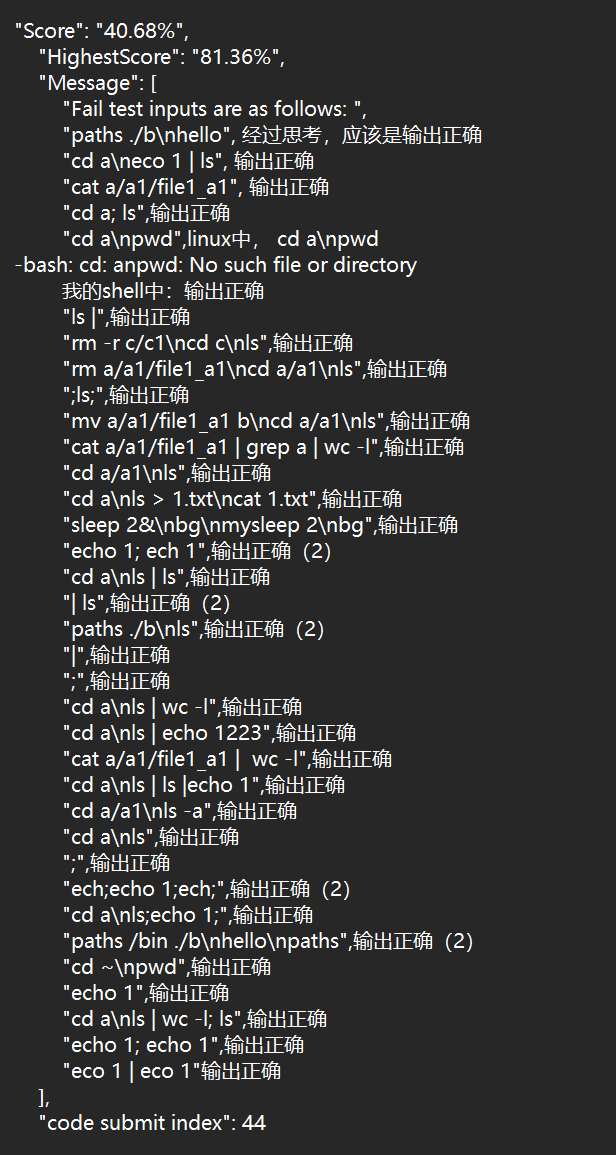
\includegraphics[width=1\textwidth]{1.png}\\
%	\caption{local test}
%	\label{fig:local test}
% \end{figure}  

\begin{document}
\title{Fat32 实验报告}
\author{221300079, 王俊童, \href{mailto:221300079@smail.nju.edu.cn}{221300079@smail.nju.edu.cn}}
\maketitle
    \section{关键问题}

    做这个fat32还真的遇到了不少的问题,从18到52到58到72到78到90到92到100,太不容易了。

    首先是fat close,这个倒是没有遇到那么多的问题,过。

    然后是fat open这个函数,这个就麻烦了。根据fat32的手册描述,我应该按照cluster,data这样的顺序去找我要找的文件在哪里,
    这里考虑到是链表类的实现,我写了一个迭代器。然后麻烦的就是去找文件,这里涉及了很多fat内部的转换,不细说,然后我处理corner case
    搞了很久,大概做完搞到58左右。

    fat pread是最麻烦的。首先是那个一个簇放不完要放到下一个簇,然后我还要在处理输入寻路的情况下,包含掉很多corner case,而且最麻烦的是
    我在pread里面返回很多有问题,根本找不到,printf出来也看不出啥,最后只能一个一个试。

    fat readdir更是麻烦,这里导致了我的代码为了实现正确需要分开处理,即$find_path_1$和$find_path$,然后衍生出了很多复制版本的函数,因为readdir
    你试过之后就知道会出现很多乱七八糟的类似于Ae,At之类的奇怪size的文件,这是要过滤的,然后还要过滤掉删除文件,在这里要考虑下一个簇的问题,相当麻烦,
    为了查这些bug找了两三天,太抽象了。
    
    \section{其余问题}

    无。AC了AC了AC了AC了AC了AC了AC了AC了AC了AC了AC了AC了AC了AC了AC了AC了!!!!!!!!!!

\end{document}